\documentclass[a4paper,twocolumn,aps,prl]{revtex4-1}

\usepackage{amsfonts}
\usepackage{amsmath}
\usepackage{geometry}
\usepackage{xcolor}
\usepackage{graphicx}
%\usepackage[subfolder,cleanup]{gnuplottex}
%\usepackage{amsthm}
%\usepackage{enumitem}
%\usepackage{wrapfig}
%\usepackage{subcaption}
%\usepackage{hyperref}
\usepackage{tikz}
\usepackage{lipsum}

% Nicer brackets for operators
\let\originalleft\left
\let\originalright\right
\renewcommand{\left}{\mathopen{}\mathclose\bgroup\originalleft}
\renewcommand{\right}{\aftergroup\egroup\originalright}

% Math operators
\providecommand{\bigO}[1]{\ensuremath{\mathop{}\mathopen{}\mathcal{O}\mathopen{}\left(#1\right)}}

% Macros
\newcommand{\diff}[3][\hspace{-0.5pt}]{\frac{\textrm{d}^{#1}#2}{\textrm{d}{#3}^{#1}}}
\newcommand{\pdiff}[3][\hspace{-0.5pt}]{\frac{\partial^{#1}#2}{\partial{#3}^{#1}}}
\newcommand{\df}{\, \textrm{d}}
%\newcommand{\eps}{\varepsilon}

% Row colouring in tables
%\usepackage[table]{xcolor}
%\rowcolors{2}{gray!25}{white}

% Margin size
\newgeometry{margin=2cm}

% Reference style
%\bibliographystyle{ieeetr}

\begin{document}

\title{Predicting NCAA March Madness 2019 with SpringRank}
\author{Brady Metherall}
\affiliation{University of Oxford}
\date{16 March, 2020}

\maketitle

\noindent
Each spring the National Collegiate Athletic Association (NCAA) hold a single-elimination tournament across the United States known as March Madness. The tournament features 68 of the top US college men's basketball teams in Division I, with the winner being crowned the national champion. The champions of each of the 32 Division I conferences automatically qualify, and the remaining 36 spots are determined by a selection committee. Since this process is done by a committee the teams given the final spots can be quite controversial. For this reason, the final eight teams selected play for four spots in what is called the First Four, which takes the field from 68 teams down to 64. We use the network ranking algorithm SpringRank \cite{debacco} to predict the outcome of March Madness 2019 games based on the scores from the regular season.

To construct our network we use the box scores of 5910 NCAA games from 2019 before March Madness began \cite{wirth}. This includes games played in all three divisions of NCAA men's basketball---a total of 649 teams. From this, we construct a directed graph and the associated adjacency matrix, where each team is represented by a node and each game is represented by an edge directed from the winner to the loser. We then compute the SpringRank from this matrix, and predict the team with the higher SpringRank to win the game.

To compute the accuracy of this prediction we compare to the actual seedings and outcomes from March Madness 2019~\cite{vanderkam}. The graph for the top 64 teams by SpringRank is depicted in Figure \ref{fig:heir}, along with how far through the tournament they advanced. Eight of the top ten SpringRank teams had a top ten seed in the tournament. SpringRank preforms well at predicting the teams that advanced to the round of 16, however, the performance decreases further down the ranking. Several teams that did not qualify for the tournament are predicted to be in the top 64 by SpringRank---this is due to the qualification process. Any team that wins their conference automatically qualifies for March Madness, but, the relative strength of each conference varies significantly. Weaker conferences must have a team represented, even though that team may be considerably weaker than a team that did not qualify from a much stronger conference. Since SpringRank only considers the relative strength of each team, many teams that were eliminated in the round of 64 are ranked below teams that were unable to qualify. Additionally, Temple and St. John's, both of whom lost in the First Four, were ranked very highly out of the teams that did not make it to the top 64, as one would expect.

\begin{figure}[tbp]
	\centering
	\begin{tikzpicture}
		\centering
		% Include figure
		\node[anchor=south west,inner sep=0] at (0,0) {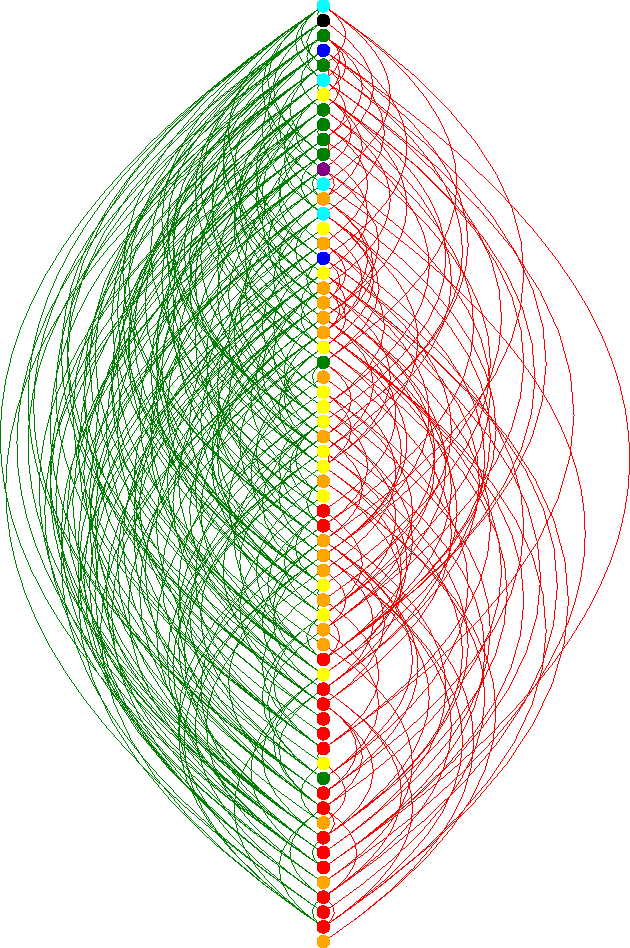
\includegraphics[width=159.22pt]{Heirarchy}};

		% Left circles
		\fill[fill = black] (0.15,1) circle (0.6mm);
		\fill[fill = {rgb,255:red,128; green,0; blue,128}] (0.15,0.667) circle (0.6mm);
		\fill[fill = blue] (0.15,0.333) circle (0.6mm);
		\fill[fill = {rgb,255:red,0; green,255; blue,255}] (0.15,0) circle (0.6mm);

		% Left names
		\node[anchor = west] at (0.25,1) {\scriptsize Winner};
		\node[anchor = west] at (0.25,0.667) {\scriptsize Runner-up};
		\node[anchor = west] at (0.25,0.333) {\scriptsize Final Four};
		\node[anchor = west] at (0.25,0) {\scriptsize Elite Eight};

		% Right circles
		\fill[fill = {rgb,255:red,0; green,128; blue,0}] (4.65,1) circle (0.6mm);
		\fill[fill = yellow] (4.65,0.667) circle (0.6mm);
		\fill[fill = {rgb,255:red,255; green,165; blue,0}] (4.65,0.333) circle (0.6mm);
		\fill[fill = red] (4.65,0) circle (0.6mm);

		% Right names
		\node[anchor = west] at (4.75,1) {\scriptsize Sweet 16};
		\node[anchor = west] at (4.75,0.667) {\scriptsize Round of 32};
		\node[anchor = west] at (4.75,0.333) {\scriptsize Round of 64};
		\node[anchor = west] at (4.75,0) {\scriptsize Did not qualify};

		% Particular teams
		\node[anchor = west] at (5,8.375) {\scriptsize Duke};
		\node[anchor = west] at (5,7.97) {\scriptsize Michigan State};
		\node[anchor = west] at (5,7.58) {\scriptsize Kansas};
		\node[anchor = west] at (5,6.13) {\scriptsize Auburn};
		\node[anchor = west] at (5,3.76) {\scriptsize Temple};
		\node[anchor = west] at (5,2.305) {\scriptsize St. John's};

		% Arrows
		\draw[->] (5,8.375) -- (2.95,8.375);
		\draw[->] (5,7.98) -- (2.95,7.98);
		\draw[->] (5,7.59) -- (2.95,7.59);
		\draw[->] (5,6.13) -- (2.95,6.13);
		\draw[->] (5,3.76) -- (2.95,3.76);
		\draw[->] (5,2.305) -- (2.95,2.305);
	\end{tikzpicture}
	\caption{Top 64 teams from SpringRank and their progress in March Madness 2019. A green (red) edge denotes a game in which the higher (lower) ranked team won.}
	\label{fig:heir}
\end{figure}

Using SpringRank to predict the winner of each game yields accuracies of $23/32$, $15/16$, $4/8$, $2/4$, $1/2$, $1/1$ for each round, respectively, and a total accuracy of $46/63 \approx 73.0\%$. The only game SpringRank incorrectly predicted in the round of 32 was when Auburn (18) upset Kansas (7) by a score of 89--75; Auburn continued on to the Final Four. Another point of interest is that the number one ranked team in the country, Duke, only made it to the round of 8. Duke (1) faced the very strong Michigan State (4), narrowly losing by a score of 67--68.

SpringRank correctly predicted the winner of $73.0\%$ of the games during March Madness 2019---a large improvement over simply guessing the winner, and a $5\%$ increase from assuming the team with the higher seed would win. Moreover, SpringRank generally predicted how well the top teams would fare, correctly predicting 14 of the teams to make the Sweet 16.

\bibliography{Ref}

\end{document}
